\subsection{Data Preprocessing}
To prepare the data several preprocessing operations were performed:

\vspace{0.2cm}\noindent
\textbf{Noise Reduction:} the audio data was already provided in a clipped format 
to minimize noise and irrelevant information.

\vspace{0.2cm}\noindent
\textbf{Normalization}: the audio are loaded using the \textit{torchaudio.load()} 
function, which normalized the audio signals in the range [-1, 1]. This is important 
to ensure that the features are on the same scale and to prevent the model from being 
biased towards features with larger values.

\vspace{0.2cm}\noindent
\textbf{Removal of Corrupted Files:} corrupted files were identified and removed 
from the dataset to ensure data quality.

\vspace{0.2cm}\noindent
\textbf{Resampling:} while literature on spoken language often suggests that 16000 Hz is sufficient, 
it was necessary to assess the best sampling rate for heartbeat sounds specifically. 
We evaluated two sampling rates to determine the optimal rate for heartbeat sounds and all audio 
files were resampled to a common frequency of 4000 Hz, 
which was identified as the optimal sampling rate (see Section \ref{sec:sampling_rate}).

\vspace{0.2cm}\noindent
\textbf{Segmentation:} the audio data was segmented into 1-second intervals, 
identified as the optimal extraction interval (see Section \ref{sec:extraction_interval}).
This segmentation allowed us to analyze the impact of different extraction intervals on model 
performance, additionally it allow for augmenting the data available. 

\vspace{0.2cm}\noindent
\textbf{Hop and Window Size}: the hop size determines the number of samples between 
successive windows, while the window size determines the number of samples considered. 
Each feature was extracted using the same window length and hop length facilitating a 
fair assessment of each feature's contribution to the classification task. 


\vspace{0.2cm}\noindent
\textbf{Outlier Detection and Removal:} we investigated the average duration of 
each class and found that the 'artifact' class had a significantly larger average 
duration. This was due to a few lengthy audio 
recordings (see Figure \ref{fig:DataExp_outliers_Artifacts}). These recordings were 
considered as outliers and removed from the dataset, as a large number of samples from 
the same audio might not be as informative.

\begin{figure}[H]
	\centering
	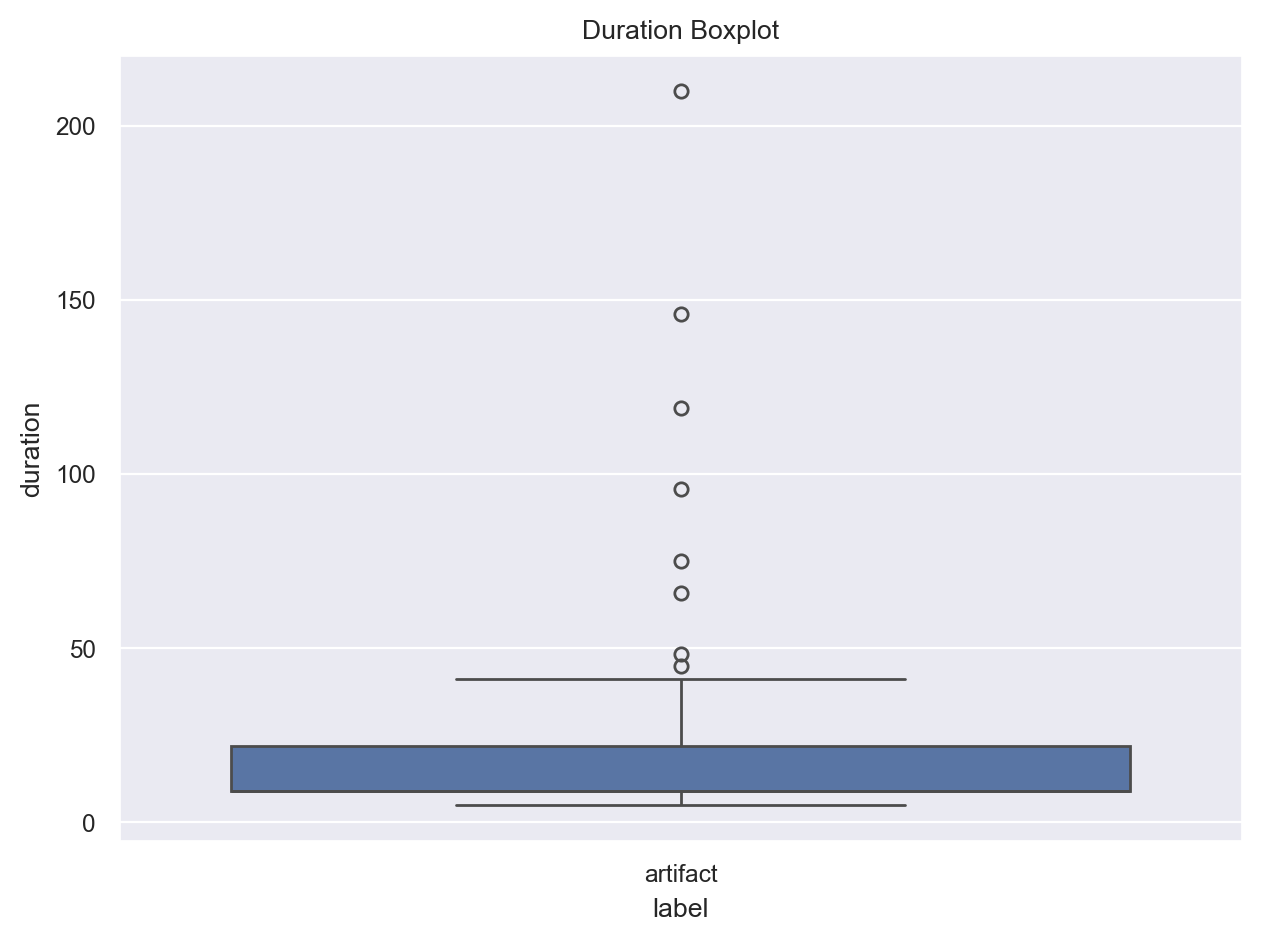
\includegraphics[width=1\columnwidth]{./images/DataExp_outliers_artifact.png}
	\caption{Outliers in the Artifacts class.}
	\label{fig:DataExp_outliers_Artifacts}
 \end{figure}\subsection{Data Preprocessing}
